\documentclass{article}
\usepackage{graphicx}
\usepackage[utf8]{inputenc}
\usepackage[T1]{fontenc}
\usepackage[english]{babel}
\usepackage{pdfpages}


\begin{document}
\title{Proposta: SLA-Guided transitions in Software Engineering}
\author{Fabio Leal}
\maketitle  

% Apresentação do problema
% Apresentação do estado da arte em transições fazendo uso do texto produzido para o artigo.

\section{Abstract}
Component-based Software Engineering (CBSE) became a popular way to develop software over the last years. During the life-cycle of a software, several components can be developed, evolved and replaced. In production environments, the replacement of a component is often a risky and delicate operation, where several factors and stakeholders take place.

Service Level Agreements (SLA), according to ITILv3's official glossary, is ``an agreement between an IT service provider and a customer. The agreement consists on a set of measurable constraints that a service provider must guarantee to its customers.''. In practical terms, it is a document that a service provider delivers to its consumers with minimum quality of service (QoS) metrics.

This work aims to assess and improve the use of SLAs to guide transition/replacement scenarios in software components, such as databases, business logic and user interface. At first, our study will focus on database transition scenarios, where we want to propose a SLA-Guided process to support migration processes from a relational database management system (RDBMS) to NoSQL. The proposed process will be validated by case studies.


\section{Background}
The goal of this chapter is to present the technical concepts for a better understanding of our job. 

\subsection{Cloud Computing \& The technological shift}

The adoption of cloud solutions is growing fast among organizations~\cite{6546068}.
Centralized (mostly mainframe) technology is being replaced by distributed and more flexible forms of data storage and processing.
This change of paradigm is motivated by the necessity to improve the use of resources, as well as by the increasing velocity in which data is produced.

In this scenario, transitions must take into account the quality of the service delivered by the new solutions.

On the early 90's it was commonplace for every Information Technology (IT) company to have its own Data Center with huge servers and mainframes. 
IT costs were high, and high-performance computing was available only for big companies, as data centers required a large physical infrastructure and have high costs for maintenance~\cite{Armbrust09m.:above}.

The regular way of building a web application was to use a client-server approach, where the server was a powerful (and expensive) machine. 
At the same time, new players, such as Google or Yahoo, were rising with bigger missions: \textit{``to organize the world's information and make it universally accessible and useful''}~\cite{Spector:2012:GHA:2209249.2209262}. 
The popularization of the internet use incentivized new ways of commerce exchange, yielding an explosion in the amount of data produced and exchanged. 
It was \textit{just} impossible to store the petabytes of daily-generated data in a single server. 

From this point on, the community realized the economical convenience of building and maintaining several low-performance servers, instead of a single high-performance one, even if this this requires a change of culture in the administration of the new datacentres.
The new approach is also incompatible with the traditional way of building applications, that usually were designed to work on a single server and database. 

Several research initiatives were conducted in this area and a common solution was rising: to distribute data storage and processing. 
Google, Yahoo and other big IT players helped to build open source tools to make this approach possible, like Hadoop~\cite{5496972}.

This revolution brought to life the notion of \textit{Cloud Computing}, together with new concepts, such as Infrastructure as a Service \textit{(IAAS)}, Platform as a Service \textit{(PAAS)} and Software as a Service \textit{(SAAS)}~\cite{AViewOfCloudComputing}.
According to~\cite{AViewOfCloudComputing}, \textit{Cloud computing refers to both the applications delivered as services over the Internet and the hardware and systems software in the data centers that provide those services.} 


\subsection{Data Integration \& Polyglot Persistence}
On the last years, the number of Data Base (DB) Engines grew like never before~\cite{dbranking}. 
Along with the NoSQL (Not only SQL) movement and expansion of Social Networks, new concepts for Database Models appeared, like Document Store, Search Engines, Key-Value store, Wide Column Store, Multi-Model and Graph DBMS. 
In~\cite{dbranking} a ranking of the most popular DB engines is presented.

Today, instead of having a single Relational Database Management System (DBMS) for the whole application, it is efficient and cost-effective to have several Data Base Engines, one for each type of data that the application handles. 
This concept is called \textit{Polyglot Persistence}~\cite{sadalage2012nosql}.

As \cite{AdressingDataManagementCloud} illustrates, polyglot persistence is very useful in the context of  e-commerce applications that deal with a catalog, user access logs, financial information, shopping carts and purchase transactions, for example.
The notion of polyglot persistence is built upon the observation that the \textit{nature} of each data type is significantly different (i.e: user logs imply high volume of writes on multiple nodes, shopping carts need high availability and user sessions require rapid access for reads and writes). 

As computing services started to decentralize, developers started to build applications that depended of several data-sources. 
By this time the use of Web Services and Service Oriented Architecture (SOA) became more popular~\cite{Armbrust09m.:above}. 


\subsection{Systematic Mappings}
According to \cite{Petersen:2008:SMS:2227115.2227123}, ``\textit{A software engineering systematic map is a defined method to build a classification scheme and structure a software engineering field of interest.}''
Systematic Mapping studies provide a global view of a given research field and identify the quantity, results, and the kinds of researches in this field.

A Systematic map is composed by a number of steps (Figure~\ref{fig:sms}).
\begin{figure}[ht!]
\centering
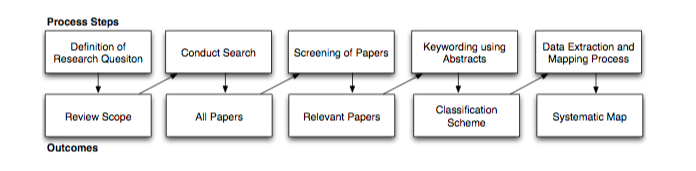
\includegraphics[width=100mm]{pic1.png}
\caption{Systematic Mapping Steps~\cite{Petersen:2008:SMS:2227115.2227123}.\label{fig:sms}}
\end{figure}

On the first step, ``Definition of Research question'', the questions that must be answered on the survey are defined. 
On the ``Review Scope'' step, researchers target the papers/journal sources that will be taken into consideration on the systematic map. 
After that, the ``Search'' step is done using a set of predefined search engines and a body of papers (``All papers'') is retrieved. 

After an initial ``Screening of the papers'', the ``Relevant papers'' are chosen according to inclusion and exclusion criteria defined by the research team. 
At this point, the papers that will participate of the study are selected. 
The selection is based on the title, abstracts and keywords of each paper (``Keywording using Abstracts'').

After that, a ``Classification Scheme'' is built, defining different points-of-view (or facets) from which the body of papers will be classified. 
After matching each paper with the classification schema (``Data Extraction and Mapping Process''), the  systematic mapping is performed.
In this phase the relationships between the collected data (in the light of the classification scheme) are used to answer the research questions.


\paragraph*{Service Level Agreements (SLAs)}
According to \textit{ITILv3's} official glossary \cite{itilv3glossary}, a Service Level Agreement (SLA) is ``\textit{an agreement between an IT service provider and a customer. 
A service level agreement describes the IT service, documents service level targets, and specifies the responsibilities of the IT service provider and the customer.}'' 

The agreement consists on a set of measurable constraints that a service provider must guarantee to its customers.
In practical terms, it is a document that a service provider delivers to its consumers with minimum quality of service (QoS) metrics. 
If the service is delivered with a lower QoS than is promised on the SLA, consumers may be refunded or earn benefits that were accorded beforehand.    

\section{Bibliographic Review}\label{bibreview}

To provide us a better understanding over the use of SLAs in component migrations, we have performed a Systematic Mapping study to assess the use of SLAs in database transition scenarios, specifically on migrations from relational databases to NoSQL ones. 

This study is available on Appendix \ref{appendix}. 
% Mudar isso para o apêndice ficar mais "real".

\subsection{Identified problems}

As a result, we have analyzed over 70 publications closely related to the use of SLAs in migration scenarios. The study revealed a number of interesting outcomes, and we emphasize two of them below:

\begin{itemize}
\item{No publication was found addressing the problem of measuring the overall improvements after a database transition. Several benchmarking frameworks, such as TPC-H, TPC-DS and YCSB were identified\cite{6616442} during our survey, though. These benchmarking frameworks could be a good starting point to develop new tools and specialized frameworks to solve this problem;
}

\item{ \cite{6253526}, \cite{6461875}, \cite{6511780} and \cite{Xiong:2011:APA:2038916.2038931} propose SLA-centric/User-Centric solutions to monitor the performance of web applications. All these solutions are technology-agnostic and could be used to monitor the performance improvements promised by a database transitioning process. Industry experts also pointed out that there are some services, such as New Relic~\cite{newrelic}, Appsee~\cite{appsee} and Datadog~\cite{datadog} that provide SLA-monitoring tools for web apps. 

The systematic mapping revealed no open source solution to monitor Application SLAs in a user-centered view (application level).  
}

\end{itemize}

\subsection{Proposed solution}

Service-Oriented Architecture (SOA) suggests that a Software Component can be seen as a set of sub-services. In the context of a Web Application, for example, it is possible to entirely replace a component just by changing the API address that it uses. This scenario of component replacement on cloud-based applications can be seen on (Figure~\ref{fig:apireplacement}).

\begin{figure}[ht!]
\centering
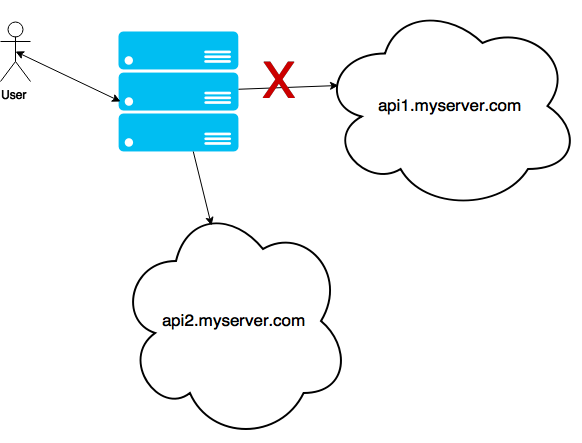
\includegraphics[width=100mm]{api.png}
\caption{Component replacement on cloud-based software.\label{fig:apireplacement}}
\end{figure}

As Section \ref{bibreview} presents, contributions can be made in the context of proposing SLA-Based and user-centered solutions to monitor component replacement scenarios. In this job, we propose the conception of a SLA-Guided process to support the migration/replacement of sotware components based on the cloud. 

We start by studying database transitioning cases, where we want to design a SLA-Guided framework to assist the migration of relational databases do NoSQL ones.

After the process is designed, we want to build an open source tool that implements the designed framework, so that it can be used by the community and validated in case studies. 

With that, our job can be summarized in three main phases:

\begin{itemize}
\item{Phase 1: Conception and design of a SLA-Based and user-centered framework to assist component migrations on cloud environments;}

\item{Phase 2: Validation of the designed framework on a database migration scenario, migrating from RDBMS to NoSQL;}

\item{Phase 3: Development of an open-source automated tool that implements the proposed framework;}

\item{Phase 4: Validation of the developed tool with case studies;}
\end{itemize}

Esqueleto do framework (estava comentado, só estou colocando para discutirmos em cima disso):
1 - Criação de SLA para cada operação disponibilizada pelo component: Nesse passo definimos um SLA que tal serviço deve obedecer (chamadas a tal endpoint devem retornar em <2s, por ex. Esse SLA servirá para “provar” que a minha tecnologia + infraestrutura atual não me atende satisfatoriamente.

2 - Criação de uma suíte de testes automatizados (ou user requests) que mostre que a aplicação não respeita o SLA acordado no passo anterior. 

3 - Proposição de nova infraestrutura/tecnologia

4 - Implementação e Simulação

6 - Comparação dos testes antigos e novos

7 - Validação da melhoria e cumprimento do SLA acordado na etapa 01.

8 - Monitoramento contínuo das operações após a migração (SLA ativo)

- A validação do framework e da app a partir de aplicações de exemplo com Open Stack;

- Open-source app que escuta todas as requisições a um servidor (JS-based e server based) e analisa se um SLA foi respeitado após alguma mudança; 

- Implementação com alguma coisa de Open Stack; 
 
\newpage
\bibliographystyle{plain}
\bibliography{fabiosmastersbib}	

\newpage
\section{Appendix}\label{appendix}
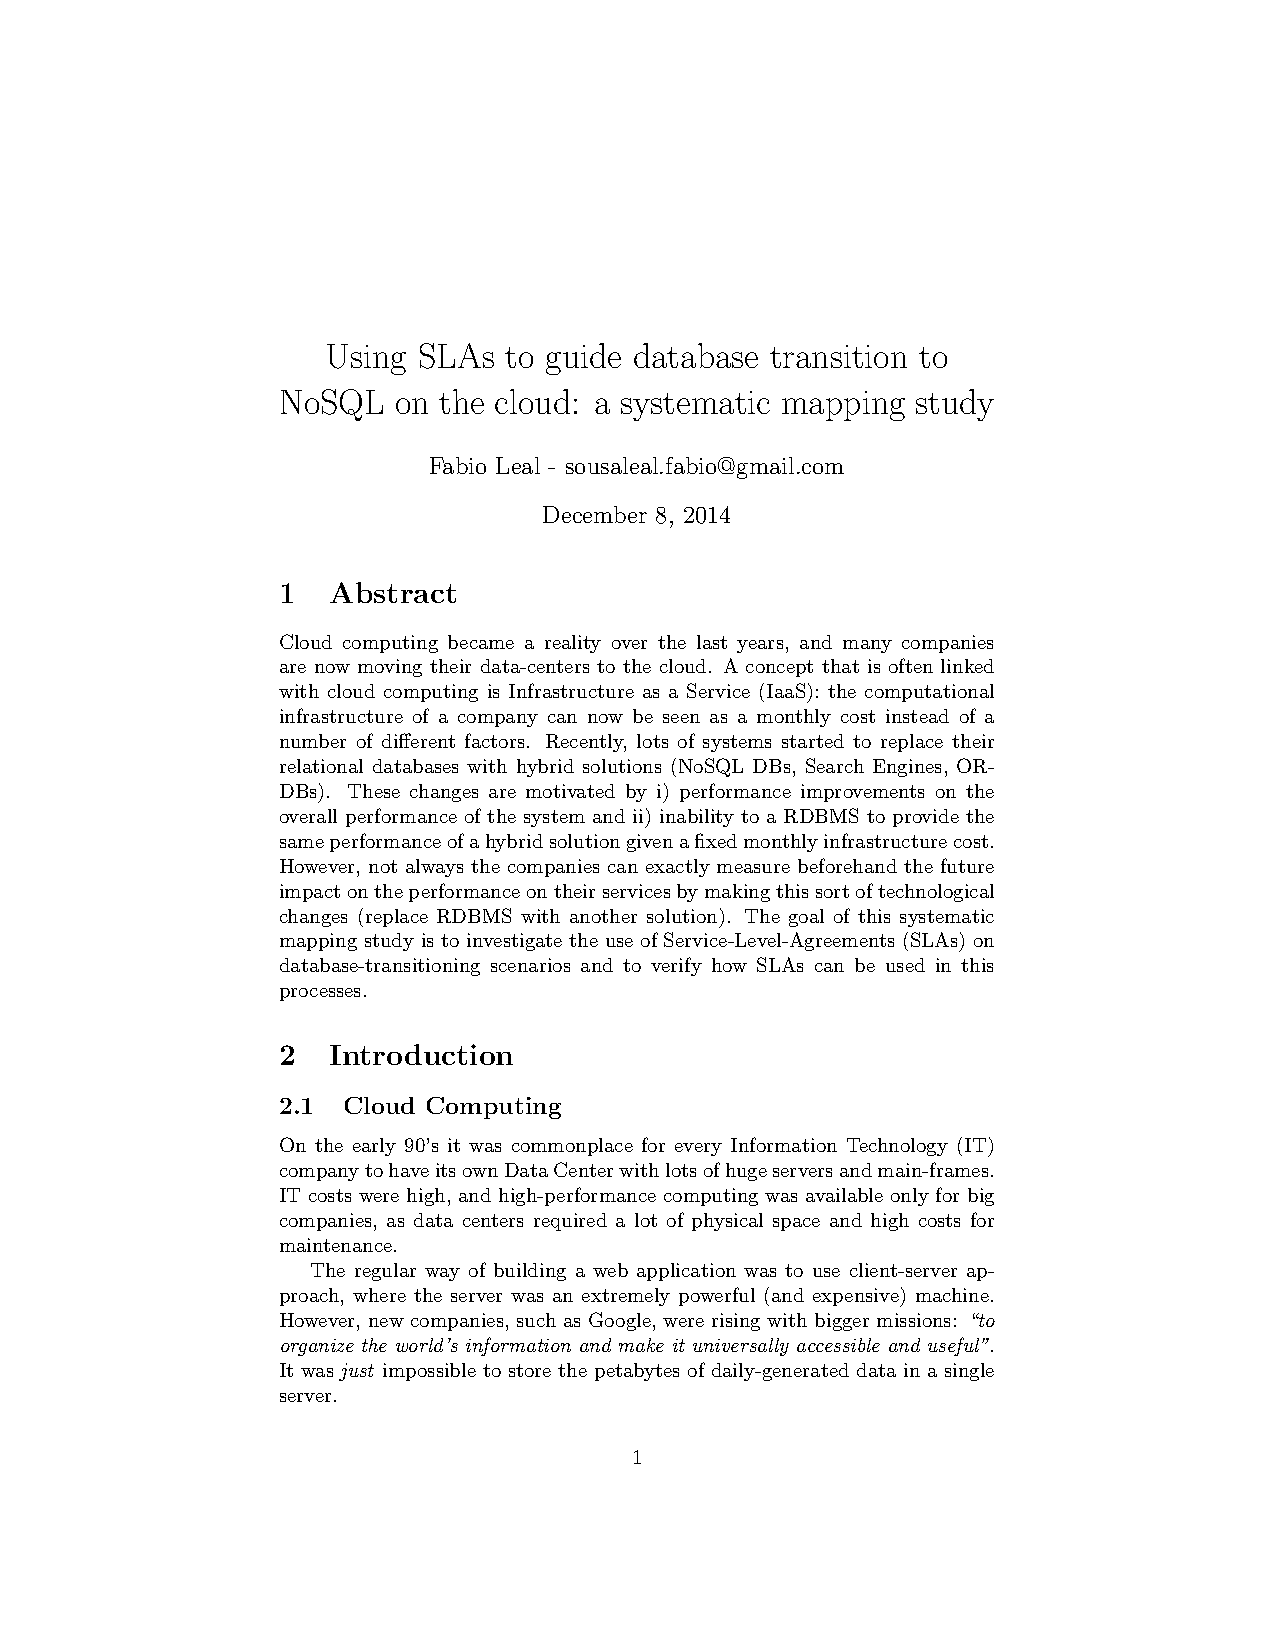
\includepdf[pages=-]{../SystematicMapping/systematicMapping.pdf}

\end{document}